\documentclass[]{article}
\usepackage{xcolor,listings}
\usepackage{textcomp}
\usepackage[margin=1.0 in]{geometry}
\usepackage{graphicx}
\usepackage{biblatex}
\usepackage{hyperref}
\usepackage{subcaption}
\usepackage{amssymb}
\usepackage{lscape}
\usepackage{rotating}
\definecolor{light-gray}{gray}{0.95}
\newcommand{\code}[1]{\colorbox{light-gray}{\texttt{#1}}}
\title{DNN model evaluation metrics}
\author{Lacey Conrad\\DNN Research\\ Regis University}
\date{July, 2021}

\begin{document}
	\maketitle
\section{General}

Public image datasets:

\url{http://www.cvpapers.com/datasets.html}

- Can reduce overfitting by adding noise.

\section{Point Cloud info}
\begin{itemize}
	\item Recent literature on point cloud models:
	
	\url{https://github.com/NUAAXQ/awesome-point-cloud-analysis-2021}
	
	\item Point cloud deep learning.  Compares different models and shows results with different datsets.
	
	\url{https://on-demand.gputechconf.com/gtc/2018/presentation/s8453-point-cloud-deep-learning.pdf}
\end{itemize}



\section{Object Detection in DNN/CNN} 
Given an image, find the objects in it, locate their position and classify them.
Object detection models are usually trained on a fixed set of classes, so the model would locate and classify only those classes in the image.
Also, the location of the object is generally in the form of a bounding rectangle.
So, object detection involves both localization of the object in the image and classifying that object.
\begin{figure}[!h]
	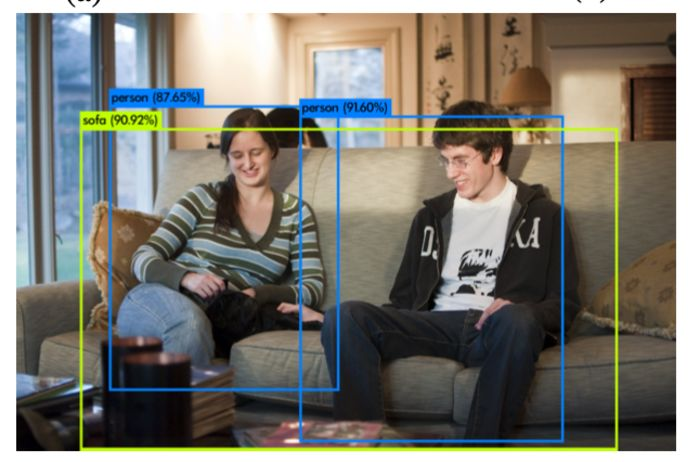
\includegraphics[scale=0.95]{bounding_boxes}
	\caption{(Wadawadagi, 2020)}
	\label{Fig:Race}
\end{figure}

\begin{figure}[!h]
	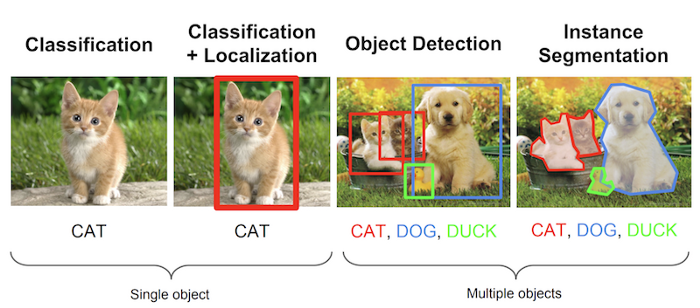
\includegraphics[scale=0.65]{obj_det}
	\caption{Common image processing problems (Shah, 2018)}
	\label{Fig:Race}
\end{figure}


\subsection{About the Ground Truth}
For any algorithm, the metrics are always evaluated in comparison to the ground truth data. We only know the Ground Truth information for the Training, Validation and Test datasets (Shah, 2018).
\pagebreak
\begin{figure}[!h]
	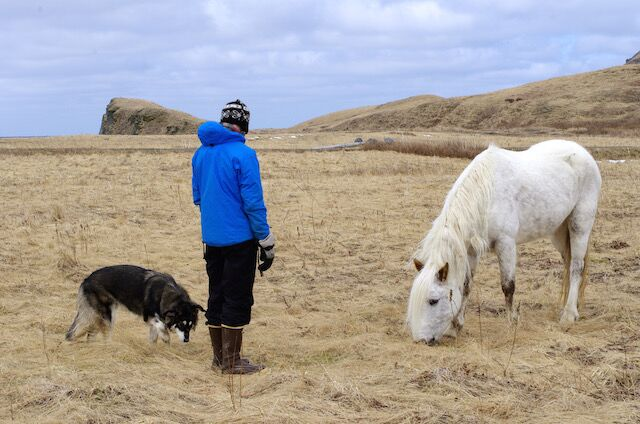
\includegraphics[scale=0.65]{ground2}
	\caption{The actual image (Shah, 2018)}
	\label{Fig:Race}
\end{figure}

\begin{figure}[!h]
	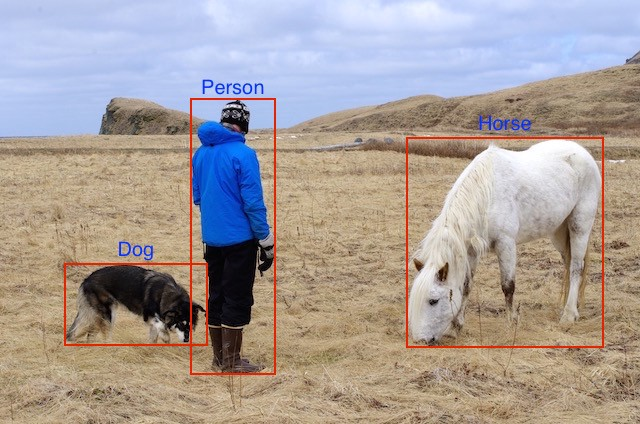
\includegraphics[scale=0.65]{ground}
	\caption{Human visualization of the ground truth (Shah, 2018)}
	\label{Fig:Race}
\end{figure}


\begin{figure}[!h]
	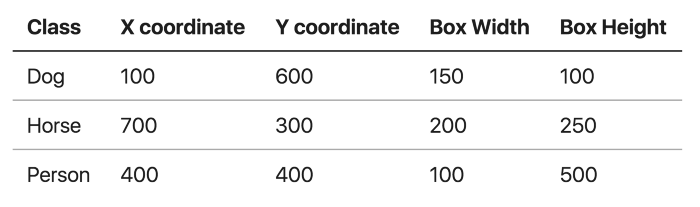
\includegraphics[scale=0.65]{ground3}
	\caption{The data defining the ground truth (Shah, 2018)}
	\label{Fig:Race}
\end{figure}

We are given the actual image(jpg, png etc) and the other annotations as text(bounding box coordinates (x, y, width and height) and the class), the red box and text labels are only drawn on this image for us humans to visualize (Shah, 2018).

\section{Working with data in neural networks}


\subsection{Edges as features}
\begin{enumerate}
\item For us to be able to see an object, the object’s color and associated properties 
must be different from the background
\item When so, the object gets a distinct boundary at overall level. Further, within the 
boundary of the object may be sub-boundaries marking separate regions such as eye
\item It is these boundaries that act as features in object detection and recognition. The main 
motive for computer vision
\item Boundaries, also known as edges are those positions in space where the characteristics 
of light change
\item Thus, detecting the changes in the light helps detect edge and edge detection is the key 
to computer vision
\end{enumerate}
\subsection{Pixel Intensity Gradient} 
\begin{enumerate}
\item Through the use of a filter function on the image function (convolution) , we try to 
detect edges. 
\item The edges appear as a gradient at a pixel (is the direction in which intensity 
changes maximum in that pixel’s neighborhood
\item The gradient is searched in both X and Y direction and a consolidated gradient is 
found using vector addition (gradients are vectors)
\item The larger the magnitude of the gradient, the stronger the evidence of presence 
of an edge / a feature
\end{enumerate}

\end{document}